\documentclass{article}
\usepackage[utf8]{inputenc}
\usepackage[margin=0.8in]{geometry}

\title{Union-Find}
\author{Justin Zhang & Daniel Wisdom}
\date{17 September 2017}

\usepackage{graphicx}

\usepackage{algorithm}
\usepackage{algorithmicx}
\usepackage[noend]{algpseudocode}

\usepackage{tikz}
\usetikzlibrary{calc,shapes.multipart,chains,arrows,positioning}

\tikzstyle{vertex}=[draw,fill=myseagreen,circle,minimum size=24pt,inner sep=0pt]

\tikzstyle{splitvertex}=[draw,fill=myseagreen,circle split,minimum size=24pt]


% for black and white printing; see below
%\definecolor{myseagreen}{RGB}{88,197,191}
%\definecolor{mysalmon}{RGB}{255,160,122}
%\definecolor{myred}{RGB}{255,102,102}
%\definecolor{mypurple}{RGB}{225,145,255}

\definecolor{myseagreen}{RGB}{238,238,238}
\definecolor{mysalmon}{RGB}{204,204,204}
\definecolor{mypurple}{RGB}{170,170,170}

\definecolor{myblack}{RGB}{0,0,0}
\definecolor{mywhite}{RGB}{255,255,255}


\begin{document}

\maketitle

\section{Union Find}
    Given an array $a$ of length $n$, with elements $1, 2, 3 ... n$, each representing a ``group," union find consists of two operations:
    \begin{itemize}
    \item \textit{union(p, q):} Connect two groups with elements at indices $p$ and $q$; change all elements in group $q$ to group $p$.
    \item \textit{find(p):} Return the group of the element at index $p$.
    \end{itemize}

    Let's formalize this concept...
\section{Connectivity}
\subsection{Connected components}
In an undirected graph, we say that two vertices are \textit{connected} if you can reach one from the other by traversing a series of edges. Then, a connected component is a subgraph such that any two vertices in the component are connected.

\begin{figure}[h]
\centering
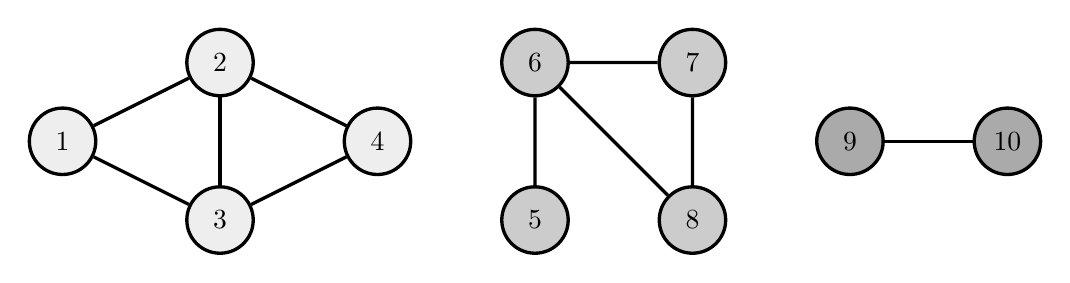
\begin{tikzpicture}[very thick,level/.style={sibling distance=70mm/#1}]
\draw (0, 0) node [vertex] (n1) {1};
\draw (2, 1) node [vertex] (n2) {2};
\draw (2, -1) node  [vertex] (n3) {3};
\draw (4, 0) node [vertex] (n4) {4};
\draw (n1) -- (n2);
\draw (n2) -- (n3);
\draw (n3) -- (n4);
\draw (n2) -- (n4);
\draw (n1) -- (n3);
\draw (6, -1) node [vertex, fill=mysalmon] (n5) {5};
\draw (6, 1) node [vertex, fill=mysalmon] (n6) {6};
\draw (8, 1) node [vertex, fill=mysalmon] (n7) {7};
\draw (8, -1) node [vertex, fill=mysalmon] (n8) {8};
\draw (n5) -- (n6) -- (n7) -- (n8) -- (n6);
\draw (10, 0) node[vertex, fill=mypurple] (n9) {9};
\draw (12, 0) node[vertex, fill=mypurple] (n10) {10};
\draw (n9) -- (n10);
\end{tikzpicture}
\caption{This diagram illustrates a graph with three connected components. \textit{Credit: Samuel Hsiang}}
\end{figure}

Determining connectivity can be done with flood fill (DFS/BFS).
Union find is concerned with the following operations (equivalent to those listed in Section 1):
\begin{itemize}
    \item \textit{find(p):} Determine which connected component a vertex $p$ is in. This is easily accomplished with flood fill.
    \item \textit{union(p, q):} Connect two vertices $p$ and $q$ in the graph.
\end{itemize}

\pagebreak

\section{Union-find (Disjoint-set)}
The goal of the \textit{union-find data structure} is to solve these two queries efficiently. Naive solutions might be to:
\begin{itemize}
    \item Represent the problem with an solely an array (Section 4). This performs \textit{find} in $O(1)$ (index lookup) and \textit{union} in $O(N)$ (iterate through the entire array to change the elements).
    \item Represent the problem with a graph or graph-based array (Section 5). This performs both \textit{find} in $O(N)$ (traverse the tree upward to find the root) and \textit{union} in $O(N)$ (change the root pointer, which requires \textit{find}).
\end{itemize}

\begin{figure}[h]
\centering
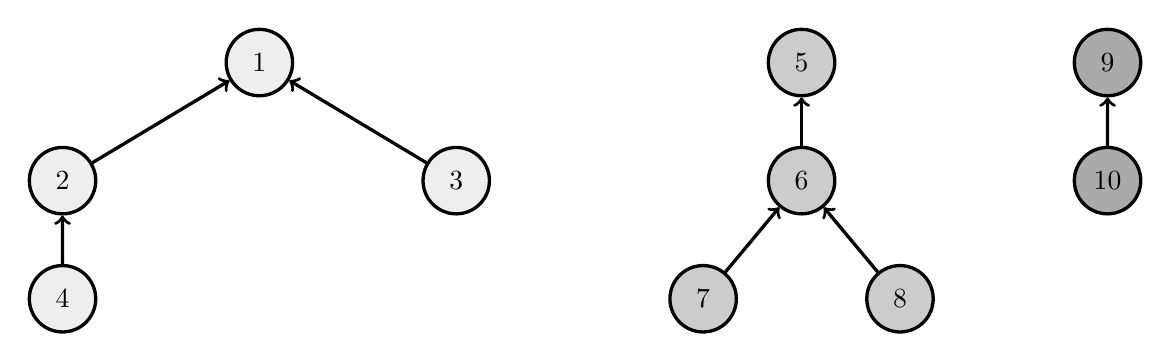
\begin{tikzpicture}[very thick,edge from parent/.style={draw,<-},level/.style={sibling distance=50mm/#1}]
\node [vertex, fill = mysalmon] (r2) {5}
  child {
      node [vertex, fill = mysalmon] {6}
      child { node [vertex, fill=mysalmon] {7} }
      child { node [vertex, fill=mysalmon] {8} }
  };

\node [vertex] [left=6cm of r2] (r1) {1}
  child {
    node [vertex] {2}
    child {
      node [vertex] {4}
    }
  }
  child {node [vertex] {3} };
  
\node [vertex, fill=mypurple] [right=3cm of r2] (r3) {9}
  child { node [vertex, fill=mypurple] {10} };
\end{tikzpicture}
\caption{Representation of union-find as a forest. \textit{Credit: Samuel Hsiang}}
\end{figure}

If we number our nodes sequentially, we can easily represent these pointers in an array instead. Instead of a null parent pointer, root nodes will point to themselves.

\begin{figure}[h]
\centering
{
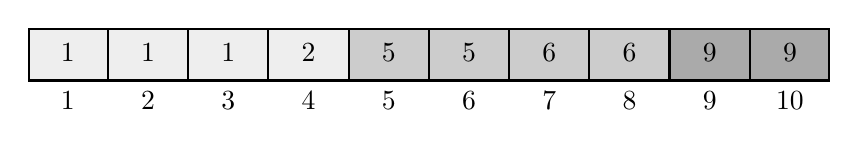
\begin{tikzpicture}[
  thick,
  myrect/.style={
    draw,
    rectangle split,
    rectangle split horizontal,
    rectangle split parts=#1,
    rectangle split part align=left,
    text width=5ex,
    text centered
    },
  mycallout/.style={
    shape=rectangle callout,
    rounded corners,
    fill=mysalmon,
    callout absolute pointer={#1},
    callout pointer width=1cm
  }  
]

\node[myrect=10, rectangle split part fill={myseagreen, myseagreen, myseagreen, myseagreen, mysalmon, mysalmon, mysalmon, mysalmon, mypurple, mypurple}]
  (array1)
  {
  					\strut 1
  \nodepart{two}	\strut 1
  \nodepart{three}	\strut 1
  \nodepart{four}	\strut 2
  \nodepart{five}	\strut 5
  \nodepart{six}	\strut 5
  \nodepart{seven}	\strut 6
  \nodepart{eight}	\strut 6
  \nodepart{nine}	\strut 9
  \nodepart{ten}	\strut 9
  };
\foreach \Valor [count=\Valori from 1] in {one ,two ,three ,four ,five ,six ,seven ,eight ,nine ,ten }
  \node[below] at (array1.\Valor south) {\Valori};

\end{tikzpicture}
}
\caption{Representation of union-find as an array. \textit{Credit: Samuel Hsiang}}
\end{figure}

\section{Quick-find}
One way to implement \textit{Union} and \textit{Find} is to have every node directly point to the root node of the component.

\begin{itemize}
    \item \textit{find(p):} Return the value at index $p$ of the array, the index of the connected component's root.
    \item \textit{union(p, q):} Search the array. For every element that contains the value $q$, replace it with $p$.
\end{itemize}

Now we have an algorithm that runs in $O(1)$ time for \textit{find}, but $O(N)$ time for \textit{union}. However, this is the same time complexity that we would get by simply performing a flood-fill every time we ran \textit{union}. We can do better.


\section{Quick-union}
With quick-find, we update every element in one connected component whenever we perform a union, which requires us to search the entire array. Instead, we can take a lazier approach and only update the pointer of the root element. This takes advantage of the interpretation of union-find as a tree.

\begin{itemize}
    \item \textit{find(p):} Follow the parent pointer of $p$ until we reach the representative element.
    \item \textit{union(p, q):} Change the parent pointer of $find(q)$ to point to $find(p)$.
\end{itemize}

Because \textit{find} needs to traverse the tree until it reaches a root element, its worst-case complexity is $O(N)$, proportional to the height of the tree. And because \textit{union} requires us to call \textit{find}, its complexity is also $O(N)$. This seems worse than Quick-find! But we can significantly improve the complexity of \textit{find} by limiting the depth of the tree.


\subsection{Weighting}
The worst-case scenario with quick-union is a very large tree that takes a long time to traverse. However, this is easy to avoid. Whenever we perform \textit{union}, if we keep track of the size of each tree, we can always join a smaller tree to the root of a larger tree, rather than the other way around.

It turns out that this optimization limits the maximum depth of any tree to $\log N$. This means that the cost of both \textit{find} and \textit{union} are now limited to $O(\log N)$, which is already a significant improvement.

\subsection{Path compression}
Intuitively, flattening the tree would make the find operation faster by shortening the number of pointers we need to traverse. So another optimization we can make is every time we perform $find(p)$, to change $p$ and all of its parents to point to its root node. This allows us to avoid traversing the same path more than once.

Combining weighting with path compression brings down the cost of \textit{find} and \textit{union} to amortized $O(\alpha(N))$, where $\alpha$ represents the extremely slowly-growing \textit{inverse Ackermann function}. For practical purposes, $\alpha(N)<5$. In fact, this is asymptotically optimal: union-find in constant time is impossible.


\section{Pseudocode}
This is a sample implementation of weighted quick-union with path compression. \textit{Credit: Samuel Hsiang}


\begin{algorithm}[H]
\caption{Union-Find}
%\label{}
\begin{algorithmic}
\Function{Find}{$v$}
	\If {$v$ is the root}
		\State \Return $v$
    \EndIf
    \State $parent(v) \gets \Call{Find}{parent(v)}$
    \State \Return $parent(v)$
\EndFunction
\Function{Union}{$u$, $v$}
	\State $uRoot \gets \Call{Find}{u}$
	\State $vRoot \gets \Call{Find}{v}$
    \If {$uRoot = vRoot$}
		\State \Return
	\EndIf
    \If {$size(uRoot)<size(vRoot)$}
    	\State $parent(uRoot) \gets vRoot$
        \State $size(vRoot) \gets size(uRoot) + size(vRoot)$
    \Else
    	\State $parent(vRoot) \gets uRoot$
        \State $size(uRoot) \gets size(uRoot) + size(vRoot)$
    \EndIf
\EndFunction
\end{algorithmic}
\end{algorithm}


\end{document}
